%--------------------
% Packages
% -------------------
\documentclass[11pt,a4paper]{report}
%\usepackage{gentium}

\usepackage[
backend=biber,
style=alphabetic,
sorting=ynt
]{biblatex}
\addbibresource{references.bib}

\usepackage[pdftex]{graphicx} % Required for including pictures
\usepackage[english]{babel} % Swedish translations
\usepackage[pdftex,linkcolor=black,pdfborder={0 0 0}]{hyperref} % Format links for pdf
\usepackage{calc} % To reset the counter in the document after title page
\usepackage{enumitem} % Includes lists
\usepackage{caption}
\usepackage{subcaption}
\usepackage{xcolor}
\definecolor{LightGray}{gray}{0.9}
\usepackage{minted}
\setminted{bgcolor=LightGray, breaklines=true, fontsize=\footnotesize}

\frenchspacing % No double spacing between sentences
\linespread{1.2} % Set linespace
\usepackage[a4paper, lmargin=0.1666\paperwidth, rmargin=0.1666\paperwidth, tmargin=0.1111\paperheight, bmargin=0.1111\paperheight]{geometry} %margins
%\usepackage{parskip}
\usepackage{titling}
\newcommand{\subtitle}[1]{%
  \posttitle{%
    \par\end{center}
    \begin{center}\large#1\end{center}
    \vskip0.5em}%
}


\usepackage[all]{nowidow} % Tries to remove widows
\usepackage[protrusion=true,expansion=true]{microtype} % Improves typography, load after fontpackage is selected

% Define a utility function to write vector symbols in bold
\newcommand{\bm}[1]{\textbf{#1}}
\newcommand{\vecsym}[1]{\bm{#1}}
% And a matrix symbol
\newcommand{\matsym}[1]{\bm{#1}}
% And a tensor symbol
\newcommand{\tenssym}[1]{\bm{#1}}


\title{Ruling out the rulers}
\subtitle{Understanding and checking for bias in skin lesion classification models}
\author{Mikkel Bjørn Goldschmidt}

\usepackage{amsfonts}
\usepackage{amsmath}
\usepackage{amssymb}
%-----------------------
% Set pdf information and add title, fill in the fields
%-----------------------
\hypersetup{ 	
pdfsubject = {Medical image analysis, XAI},
pdftitle = {Ruling out the rulers},
pdfauthor = {Mikkel Bjørn Goldschmidt}
}

\renewcommand\sectionmark[1]{\markright{\thesection.\ #1}}

%-----------------------
% Begin document
%-----------------------
\begin{document}
\maketitle

\tableofcontents
\pagebreak
\chapter{Introduction}
Image analysis can be used in the diagnosis of diseases in different ways.
A lot of the data used for diagnosing come in the form of images.
Examples of these are MRI, CT, PET, ultrasound but also just plain images of body parts.
Understanding these images is often done using machine learning models in different forms.
In their nature, these models are not easy to understand and can therefore end up biased without
the model designer knowing it.

This project focuses on the HAM10000 dataset\cite{Tschandl_2018}, which contains images of skin lesions.
Doctors diagnose these lesions into different classes, some more dangerous than others.
The challenge on the HAM10000 dataset is to find a model that can predict the class of a given image.

\subsection{Biases in the data}
Many different models have been trained to diagnose lesions based on medical images.
These images are taken in a real world medical context, which can introduce unknown bias into the models.
It has even been reported that models trained on medical data where the lesions were masked out,
% THIS IS NOT TRUE! 73% percent refers to AUC not accuracy.
could reach an accuracy of $73\%$\cite{DeConstructing_Bias_on_Skin_Lesion_Datasets_2019}, indicating that there are other factors in the data, 
that can be used to classify the models than the actual lesion.
Some research has tried to introduce foreign object into the images,
and found that they changed the classification of the lesions \cite{Towards_Explainable_Classifiers_Using_the_Counterfactual_Approach_2019}.
These foreign objects included ruler markings, black frames and colored circles.

\section{The HAM10000 dataset}
The HAM10000 dataset contains 10015 images of skin lesions.
These images are a subset of the images from the ISIC dataset\cite{ISIC_Dataset_2018},
which collects images of skin lesions and hosts annual competitions for skin lesion diagnosis.
They are divided into seven classes as seen in the Table \ref{table:ham10000}.
A \textit{severity} has also been assigned each class.
These indicate if the lesion class benign, malignant or pre-malignant.
Malignant tumors are those where the cells are replicationg uncontrollably,
and there is a risk of these cells spreading to the rest of the body.
Beningn tumors can still hurt the patient, but are much less of a worry,
as they are not replicationg uncontrollably and hence do not lead to cancer.

\begin{table}[ht]
\begin{center}
\begin{tabular}{|c|c|c|c|c|c|c|}
\hline
Label    & Name                          & Severity      & Dataset prevalence \\ \hline
akiec    & Bowens disease                & pre-malignant & $3.27\%$           \\ \hline
nv       & Melanocytic nevi              & benign        & $66.94\%$          \\ \hline
mel      & Melanoma                      & malignant     & $11.11\%$          \\ \hline
bkl      & Benign keratosis-like lesions & benign        & $10.97\%$          \\ \hline
bcc      & Basal cell carcinoma          & malignant     & $5.13\%$           \\ \hline
vasc     & Vascular lesions              & benign        & $1.41\%$           \\ \hline
df       & Dermatofibroma                & benign        & $1.14\%$           \\ \hline
\end{tabular}
\end{center}

\caption{Overview of the HAM10000 dataset.}
\label{table:ham10000}
\end{table}

\subsection{State of the art models}
Due to the public nature of the dataset, many different models have been trained on it.
As of the time of writing, the best performing model published in a scientific paper,
reaches an accuracy of $93.4\%$\cite{datta2021soft}.

\subsection{Confounding elements in the data} \label{sec:confounding}
The dataset contains images of skin lesions, which are taken in a real world medical context.
In this context doctors might introduce foreign objects into the images,
to help in the treatment of the patient.
Examples of these can be seen on Figure \ref{fig:confounding_objects}.

\begin{figure}[ht]
    \begin{center}
        \begin{subfigure}[b]{0.3\textwidth}
            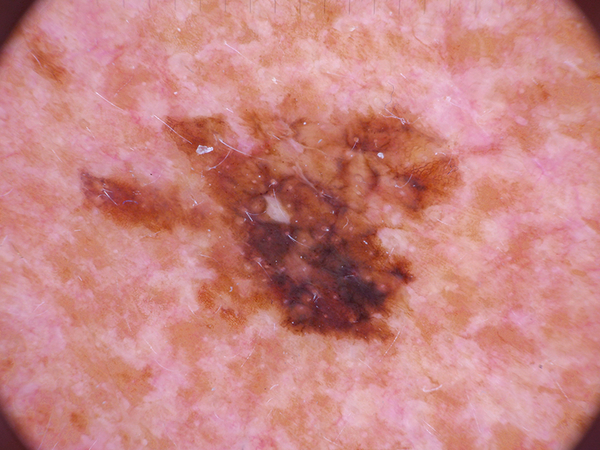
\includegraphics[width=\textwidth]{./images/ISIC_0024310.jpg}
            \caption{Image with black frame}
        \end{subfigure}
        \begin{subfigure}[b]{0.3\textwidth}
            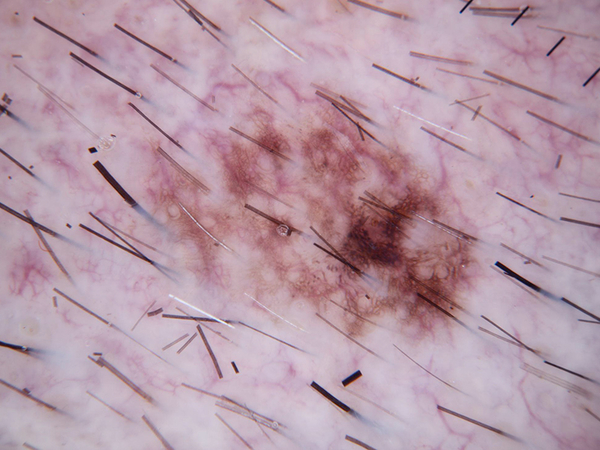
\includegraphics[width=\textwidth]{./images/ISIC_0024420.jpg}
            \caption{Image with ruler}
        \end{subfigure}
        \begin{subfigure}[b]{0.3\textwidth}
            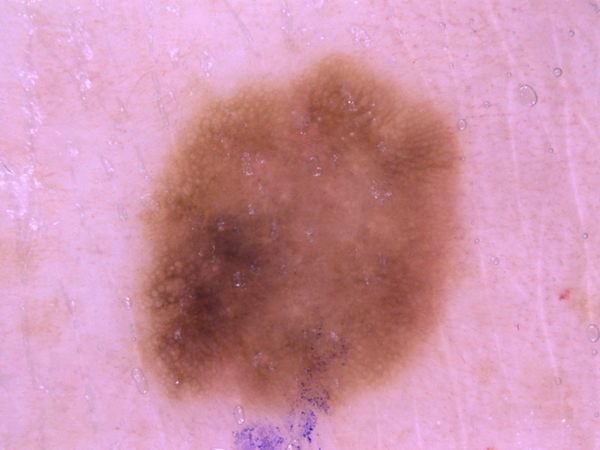
\includegraphics[width=\textwidth]{./images/ISIC_0027514.jpg}
            \caption{Image with blue ink}
        \end{subfigure}
    \end{center}
    \caption{Images with different confounding objects}
    \label{fig:confounding_objects}
\end{figure}

Labeling some of these confounding objects, we see that the rulers occur way more often than the others with a prevalence of roughly $17\%$ (See Table \ref{table:confounding_objects}).
Due to this higher prevalence, the study done in this project will focus on the ruler markings over the other confounding objects.

\begin{table}
    \centering
    \begin{tabular}{|l|r|}
        % confounding_objects.ipynb
        \hline 
        Confounder &  Prevalence \\ \hline
        ruler   &  0.171842 \\ \hline
        sticker &  0.000100 \\ \hline
        ink     &  0.003495 \\ \hline
    \end{tabular}
    \caption{Dataset prevalence of confounding objects}
    \label{table:confounding_objects}
\end{table}

\subsection{Correlation between confounding elements and HAM10000 labels}
On Figure \ref{fig:ruler_vs_dx} indications of correlations between the ruler markings and the HAM10000 labels can be seen.

\begin{figure}[ht]

\centering
\includegraphics[width=0.8\textwidth]{./build/confounder_label_correlation/confusion_matrix_seaborn.png}
\caption{Confusion matrix of rulers vs. class in the HAM10000 dataset - normalized over the x-axis.}
\label{fig:ruler_vs_dx}
\end{figure}

The two benign classes \textit{mel} and \textit{bkl} are both over represented on pictures with ruler markings copared to those without.
In general almost every class except the biggest \textit{nv} class is over represented.
The hypothesis that the presence of rulers in the images is correlated with the HAM10000, can be confirmed by a $\chi^2$-contingency test.
The null hypothesis of this test is that the presence of rulers in the images is not correlated with the HAM10000 labels.
The test value is 
    $\input{build/confounder_label_correlation/chi2.txt}$
on a test with
    $\input{build/confounder_label_correlation/dof.txt}$
degrees of freedom, resulting in a $p$-value of 
    $\input{build/confounder_label_correlation/p.txt}$
which is obviously significant.


\chapter{Model}
The initial goal of this project was to look into methods to not use ruler presence in the
diagnosis classification.
To be able to do this, a model that was using the ruler presence in its predictions was needed.
Preferably this model should also perform close to the best performing model, to be comparable.

\section{ResNet18 architecture trained with MixUp}
On the Kaggle classification competetion related to the HAM10000 dataset\cite{HAM10000-kaggle-competetion},
another user claimed to get a $97.7\%$ accuracy using a ResNet18 model trained with MixUp\cite{kaggle-97-model}.
When the provided model was retrained, the results were not as good as claimed.
The actual accuracy was in the range of $90\%$ to $92\%$, depending on the data split.
That is however still close to the best performing model published (see \ref{sec:state-of-the-art}).

The actual implementation of the model can be seen in Appendix \ref{appendix:resnet-18-mixup}.
Using the slight modifications to the original mode, the model reached an accuracy of roughly $91\%$.

\subsection{Model analysis}
\subsubsection{Prediction saliency map}
As described in the Introduction section, there is an academically described risk,
that the model will use the presence of rulers in its predictions. % Maybe a reference here?

We will first test this, by creating saliency maps (\ref{sec:saliency_maps}) for some of the images with rulers in the dataset.
These can be seen in Figure \ref{fig:ruler_saliency_map}.
More similar examples can be seen in Appendix \ref{appendix:ruler_saliency_maps}.

\begin{figure}[h]
    \includegraphics[
        width=\textwidth,
        height=\textheight,
        keepaspectratio=true,
        angle=0,
        clip=false
    ]{build/saliency_maps/overview_map_2.png}
    \caption{Saliency maps of the model prediction on an image with a ruler.}
    \label{fig:ruler_saliency_map}
\end{figure}

\subsubsection{Prediction precision on different classes}
To further evaluate the model, we will investigate wether it underperforms on some classes.
In Figure \ref{fig:prediction_strength} a confusion matrix for the trained model is shown.

\begin{figure}[ht]
    \centering
    \includegraphics[
        width=0.7\textwidth,
    ]{build/prediction_strength/confusion_matrix_seaborn.png}
    \caption{Confusion matrix of the model prediction on the dataset. 
        Normalization has been done over the truth.
    }
    \label{fig:prediction_strength}
\end{figure}

The confusion matrix shows that the model underperforms on the \verb|mel| (melanoma) class.
For terms of the using this model in practice, this would be problematic and should be adressed.
The model does however perform fairly well in general, so it will still be used to investigate the
impact of confounding elements on its predictions.

\subsubsection{Prediction strength on the melanoma class}
Assuming that the rulers do indeed affect the models predictions,
it would likely impact the prediction strength of the model if rulers are present. 
Since the rulers are overly present in the images of lesions with melanoma,
it would under the assumption be expected, that the presence of the rulers improves the model's predictions 
on the \verb|mel| class.

To test this, a plot has been created below that shows the prediction strength of the model on the \verb|mel| class,
seperated over the presence of rulers.

\begin{figure}
    \centering
    \begin{subfigure}[h]{0.45\textwidth}
        \includegraphics[
            width=\textwidth,
        ]{
            build/prediction_strength/mel_confusion_matrix_seaborn.png
        }
        \caption{No normalization}
        \label{fig:prediction_strength_mel}
    \end{subfigure}
    \begin{subfigure}[h]{0.45\textwidth}
        \includegraphics[
            width=\textwidth,
        ]{
            build/prediction_strength/mel_confusion_matrix_seaborn_normalized.png
        }
        \caption{Normalized over the presence of rulers}
        \label{fig:prediction_strength_mel_normalized}
    \end{subfigure}
    \caption{Confusion matrix of the model prediction the melanoma cases split up by presence of a ruler.}
\end{figure}


\end{figure}
\section{Debiasing Skin Lesion Datasets and Model. Not So Fast}\label{sec:debias-not-so-fast}
In their paper
''Debiasing Skin Lesion Datasets and Model. Not So Fast''
Bissoto, Alceu and Valle look into debiasing models trained on
skin lesion images \cite{debias-not-so-fast}.
They go through $7$ different artifacts in the images that could
be confounding elements, and try state-of-the-art methods to
make them disregard the artifacts.
These include the rulers, that is the focus of this report.
The paper makes several claims about biases that occur in
their skin lesion classification models.
Their focus is the removal of these bias, but the relevance to this project is that they
make claims about their models actually being biased.

\subsection{Arguments that the model is using the artifacts}
The researchers trained multiple different models to detect if the
images contained malignant or benign lesions.
Note that this classification is a simplified version of the classes
that is used in this report, as they only focus on whether a lesion is malignant or benign.
The researchers used the RESNET-18 architecture, as the basis for all their models.
They then utilize that the architecture is set up in a way where first a set of features
are extracted from the images using convolutional layers, and then fed into a fully connected layer. 
An outline of this is shown on Figure \ref{fig:resnet-outline}.

\begin{center}
    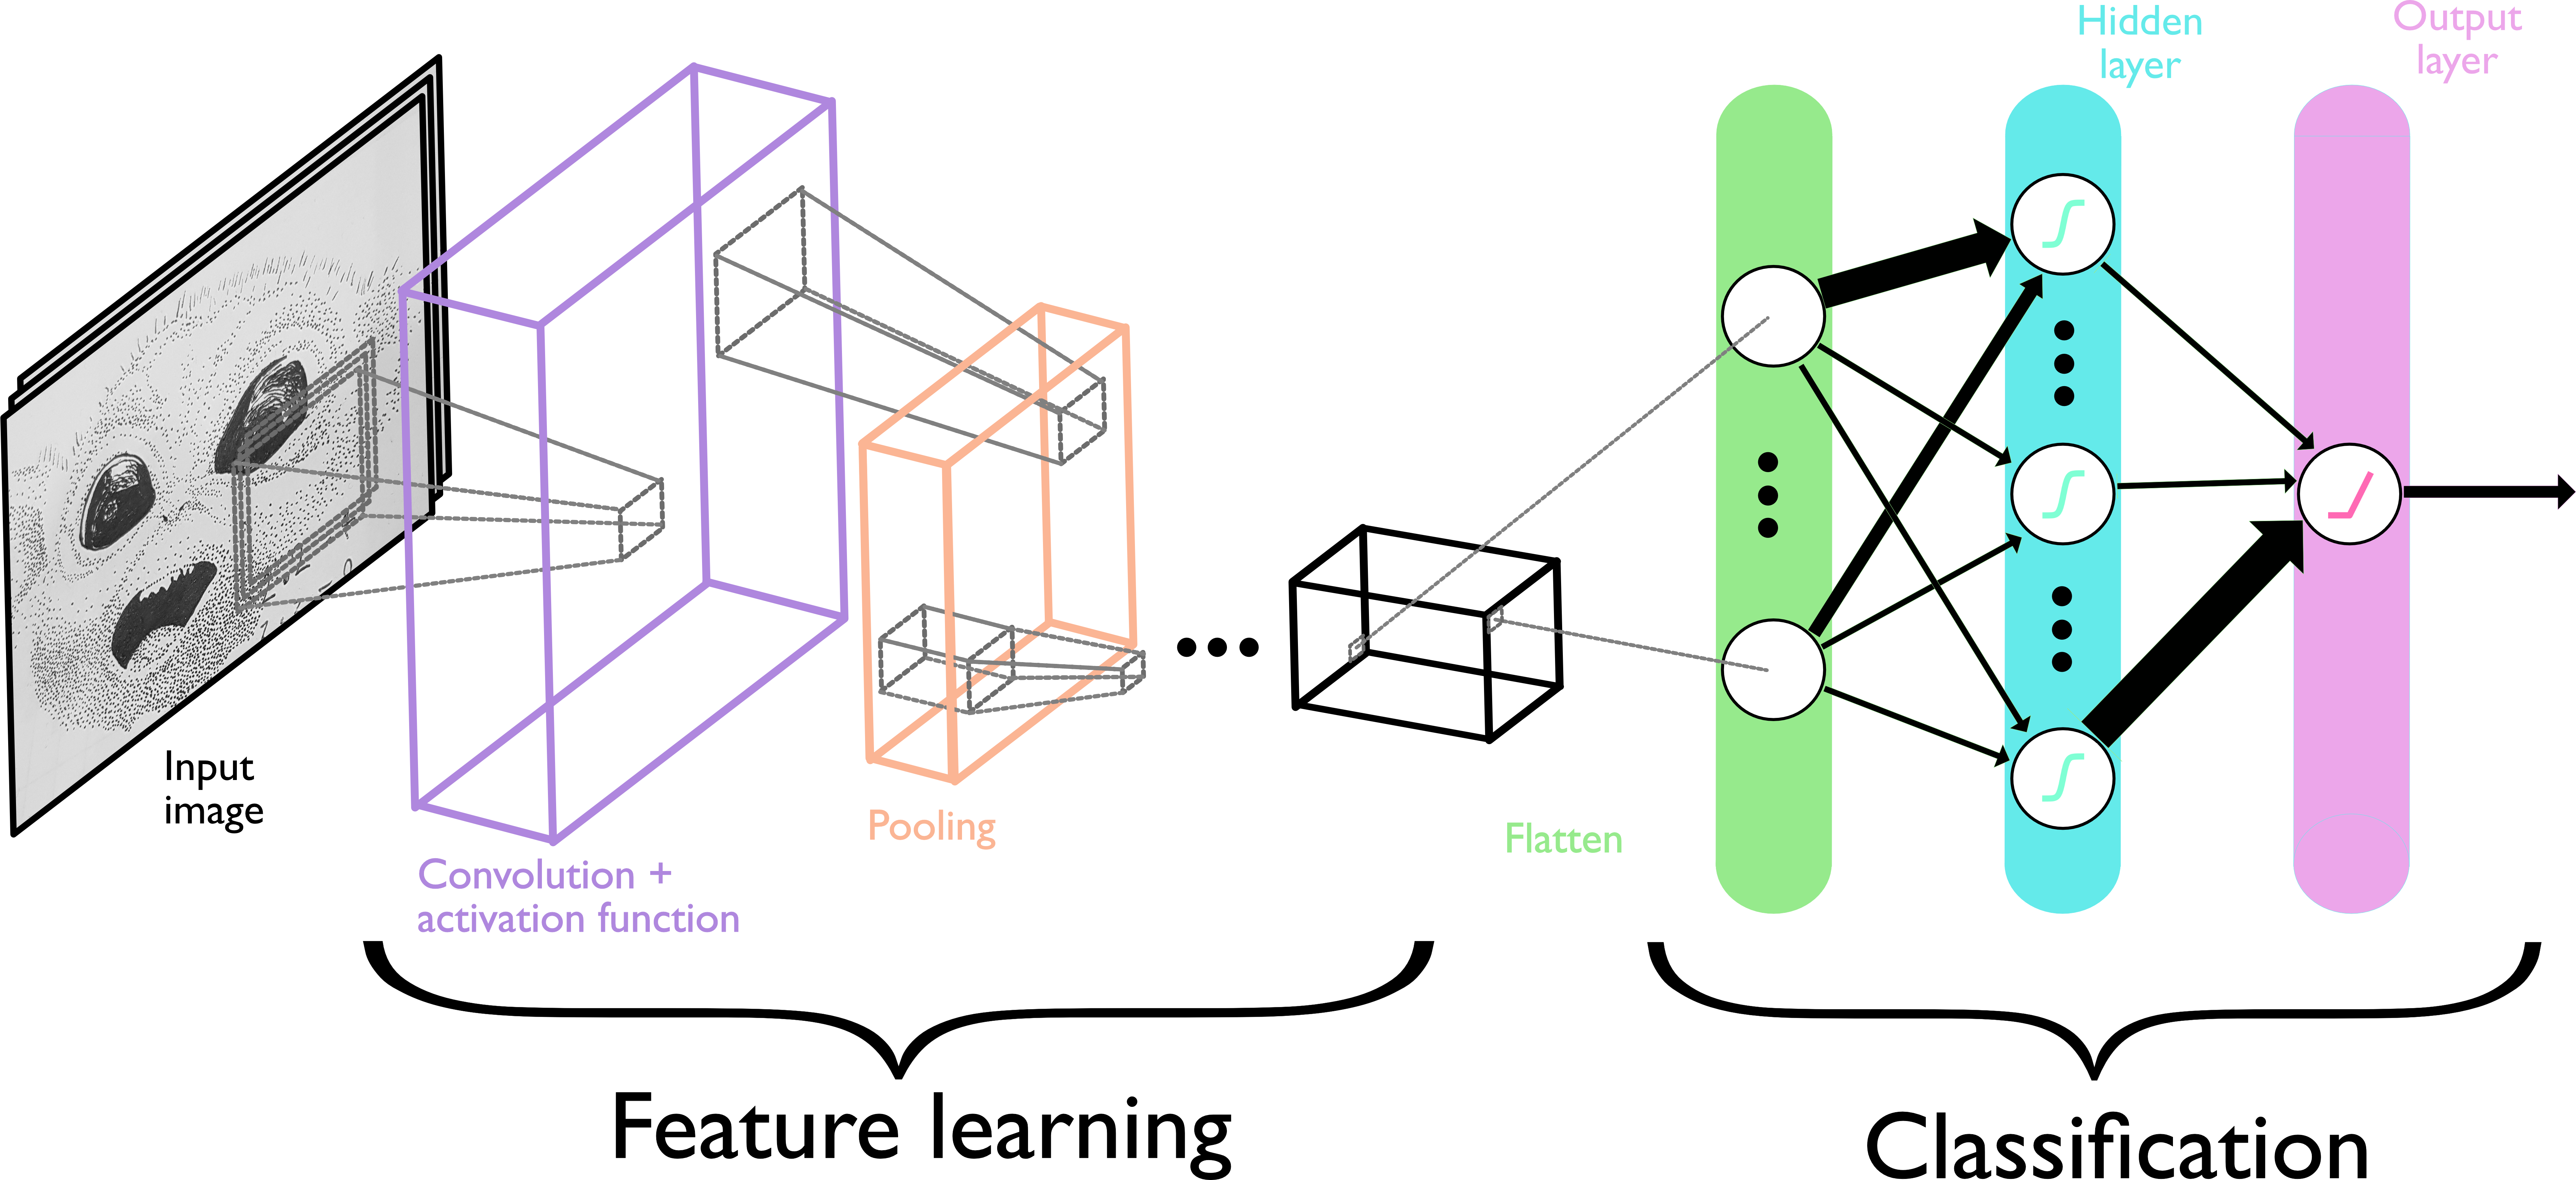
\includegraphics[width=0.9\textwidth]{images/ConvNet_V2.png}
    \captionof{figure}{A simplified view of how CNNs in general are structured with
                       convolutional layers first that extract features and fully connected layers
                       at the end to handle the classification.
                       This figure is borrowed from my wonderful writing partners \cite{alex-og-felix}.
    }
    \label{fig:resnet-outline}
\end{center}

As shown in the figure, the convolutional layer outputs a tensor (for definition of tensors, see Section \ref{sec:tensor}).
This tensor can then be converted into a vector, which can be interpreted as a feature vector for the image.
Intuitively, two images with \textit{similar} elements in the image should have a similar feature vector.
Utilizing this idea, the researchers calculate these vectors for the entire test dataset.
They then find that there is a relatively small euclidean distance between the feature vectors of images
that contain the same artifacts.
They show this by finding the nearest neighbors (with the distance measure between images being the euclidean distance between their feature vectors)
of different images artifact, and find that these neighbors often contain the same artifacts.
Their results are shown in Figure \ref{fig:not-so-fast-artifact-query}.


\begin{center}
    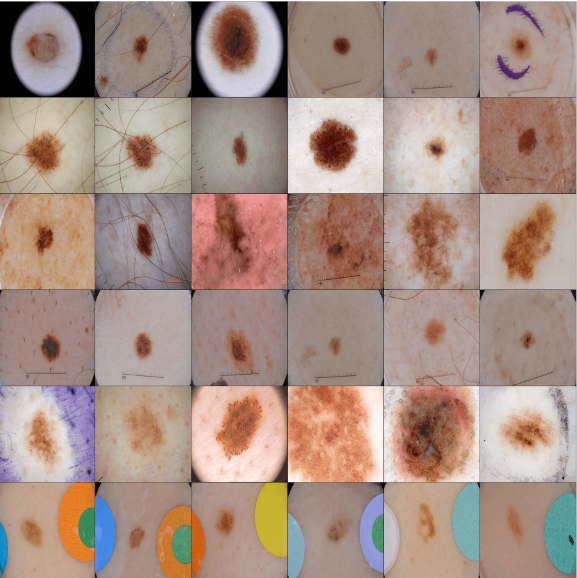
\includegraphics[width=0.4\textwidth]{images/not-so-fast-artifact-query.png}
    \captionof{figure}[Figure 4.a from \cite{debias-not-so-fast}]{
            Figure 4.a from \cite{debias-not-so-fast}, original description: \textit{Grid showing image similarity according to the features extracted by our classification model. The first column
            of each grid is the query, and the remaining columns are ranked according to euclidean distance of the images features.
            We selected queries carefully to show different artifacts.
            In sequence, dark corners, hair, gel border, ruler, ink markings and patches}}
    \label{fig:not-so-fast-artifact-query}
\end{center}

From the fact that the feature vectors of the images with the same artifacts are relatively small,
they conclude that the model is biased towards the artifacts - since the features it extracts seem to contain information about the artifacts.
The paper then goes on to examining how to mitigate these biases, but this is not relevant to this report.

\pagebreak
\chapter{Theory}
This report assumes that the reader is familiar with the basics of machine learning.
This includes basic linear algebra, data preprocessing and model selection.
Further, understanding of how neural networks function is assumed,
including the basic concept of gradient descent used for model training.

The theory described in this section is what is directly relevant to the analysis.
Some concepts that are not directly used in analysis,
but needed to understand parts of the theoretical background,
have been moved to Appendix \ref{sec:background-theory}.
The chosen theory is focused on the parts used for explainable AI, more than the technical details of how neural networks work.
In addition, a small introduction to the domain knowledge of skin lesion diagnosis is given.

\section{Lesions of the skin}
Skin lesions are parts of the skin,
that have abnormal amounts of growth compared to the surrounding skin \cite{dermatologi-laerebogen}.
In medical science, they categorize these into subcategories,
that can be treated in different ways.
Such a category can be considered \texit{malignant} or \texit{benign}.
A malignant lesion is cancerous and thus a lot more dangerous than the non-cancerous benign ones. 
The most common type of malignant lesion is \texit{melanoma}. 
In practice some lesions might be classified as \textit{pre-malignant},
like the Bowen's disease,
that is cancerous but easily treatable \cite{nhs-bowens-disease}.

Using a skin biopsy,
a doctor can precisely identify the type of a lesion.
This is done by removing a small skin sample and looking at it under a microscope.

Due to the time and cost of the biopsy,
a pre-evaluation of a lesion is needed to determine if it is likely to be malignant.
Doctors use methods like the ABCD method,
that is looking at Asymmetry, Border irregularity, Color variation and Diameter ($>6\text{mm}$)\cite{dermatologi-laerebogen}.
It is this presevaluation process that a computer can be used to help doctors spend less time,
by trying to make a prediction only based on an image of the lesion.

\subsection{Classification problems}\label{sec:classification-problems}
The classification problem as a data scientist can therefore be either the binary classification problem,
where the model is trying to predict if a lesion is benign or malignant.
For these binary problems, we will consider pre-malignant lesions as malignant,
as we in a medical context would like a doctor to be aware that treatment is necessary.

It can also be the multi-class classification problem,
where the model is attempting to predict the exact kind of a lesion.
Both of these are discussed in this report.

\section{Model metrics} \label{sec:model_metrics}
To compare the performance of models, different kinds of metrics can be used.
As mentioned in Section \ref{sec:classification-problems},
researchers tackle two different kinds of classifications.
To enable comparison with as many other studies as possible,
we will report different metrics
on both problems as described in the following.
All of the metrics are in the $\[0, 1\]$ interval with $0$ being the worst score and $1$ being the best.

\subsection{Multi-class Accuracy}
Accuracy is the percentage of predictions that are correct.
\[
    \text{Accuracy} = \frac{\text{correct classifications}}{\text{total predictions}}
\]
Accuracy as a metric is not that good for problems with big class imbalance,
such as this one where a single class accounts for more than half of the data,
which is the case in the HAM10000 dataset that is used in this report (see Table \ref{table:ham10000}).

\subsection{Binary Accuracy}
The binary accuracy is defined exactly as the multi-class, but except of using all classes,
the considered classes are just benign and malignant.
Obviously, that means what $\text{Binary Accuracy} > \text{Multi-class Accuracy}$.

\subsection{Malignant recall}
The general definition of recall in a binary classification problem is the percentage of the positive class
that is correctly classified.
The recall is defined as
\[
    \text{Recall} = \frac{\text{TP}}{\text{TP} + \text{FN}}
\]
Here $TP$ is the number of true positives, and $FN$ is the number of false negatives.
When referring to \textit{malignant recall}, we will think of the recall metric in the problem
where the considered classes are just benign and malignant.
As the name suggest, the positive class is malignant.

An intuitive way of thinking about this is how big a portion of the malignant lesions
that the model was able to detect.
On its own, a very high malignant recall does not mean the model is excellent,
as one can trivially, make it $1$ by just having a model that always predicts malignant, no matter the image.

\subsection{Malignant F1 score}
For the binary \textit{malignant vs. benign} problem, we would like to have a general score 
that takes class imbalance into account.
For this purpose, the F1 score is often used.
In general, the F1 score is defined as
\[
    \text{F1 score} = \frac{2 \cdot \text{Precision} \cdot \text{Recall}}{\text{Precision} + \text{Recall}}
\]
giving rise to the need of for positive class, as the definition of recall requires one.
Here, the \textit{Malignant F1 score} is defined as
\[
    \text{Malignant F1 score} = \frac{2\cdot \text{Precision} \cdot \text{Malignant recall}}{\text{Precision} + \text{Malignant recall}}
\]

A benefit of the F1 score is that it is a good metric to compare the performance of different models,
as it both takes the class imbalance into account,
but also just the general performance of the model.

Malignant recall is usually referred to as \texit{sensisivity} in medical literature
\cite{sensitivity-and-specificity}.

\subsection{Multi-class F1 score}
Defining a multi-class F1 score, is a bit more complicated than for a binary one.
The Python package that is used to calculate the F1 score in this project, \verb|sklearn|
\cite{sklearn}, has a mandatory parameter \verb|average|, that changes the way the F1 score is calculated.
In Figure \ref{fig:sklearn-f1-average-docs} the average parameter is described.
In this project, we will use \verb|average='weighted'|, where the F1 score is calculated
individually for each class in the problem as a positive class,
and then doing a weighted average of them based
on the number of samples in each class.
The reason for this choice,
is that it explicitly considers the class imbalance,
which is important for the multi-class problem on the HAM10000.


\begin{center}
    \begin{minted}{text}
    average : {'micro', 'macro', 'samples','weighted', 'binary'} or None, \
            default='binary'
        This parameter is required for multi-class/multi-label targets.
        If ``None``, the scores for each class are returned. Otherwise, this
        determines the type of averaging performed on the data:

        ``'binary'``:
            Only report results for the class specified by ``pos_label``.
            This is applicable only if targets (``y_{true,pred}``) are binary.
        ``'micro'``:
            Calculate metrics globally by counting the total true positives,
            false negatives and false positives.
        ``'macro'``:
            Calculate metrics for each label, and find their unweighted
            mean.  This does not take label imbalance into account.
        ``'weighted'``:
            Calculate metrics for each label, and find their average weighted
            by support (the number of true instances for each label). This
            alters 'macro' to account for label imbalance; it can result in an
            F-score that is not between precision and recall.
        ``'samples'``:
            Calculate metrics for each instance, and find their average (only
            meaningful for multilabel classification where this differs from
            :func:`accuracy_score`).
    \end{minted}
    \captionof{figure}[Cutout from sklearn documentation for F1 score]{
        Documentation for the required \textit{average} parameter for the F1 score in a multi-class problem
        (Copied from \url{https://scikit-learn.org/stable/modules/generated/sklearn.metrics.f1_score.html
        })}
    \label{fig:sklearn-f1-average-docs}
\end{center}

\section{Saliency maps}\label{sec:saliency_maps}
When training deep neural networks,
it is difficult to know exactly what the model is doing.
Especially in fields like medical image analysis,
where the classification of a model might influence if a patient is correctly diagnosed or not,
it is very desirable to know what the model is doing to be able to critique its predictions.

In image analysis, a tool to try to understand models are the so-called \textit{saliency maps}.
A saliency map is supposed to be a visual representation of what parts of the image are influential on the model,
when it made a given prediction.
In Figure \ref{fig:interps-are-useful-saliency-maps} a saliency map over a skin lesion is shown. 

For instance, in a model supposed to classify if a picture of a bone is broken or not,
it is desirable that the model looks at the bone and not really, anything else in the image.

Many methods exist to produce saliency maps, each with their own strengths and weaknesses.
One of the most popular ones is the gradient-based method (explained below).
This method is popular because it is computationally efficient,
and the implementation comes almost for free if back propagation is implemented.

\subsection{Class specific gradient-based saliency maps} \label{sec:gradiant_saliency_maps}
As described in Section \ref{sec:partial_derivatives_of_scalar_over_vector},
if a function $f: \mathbb{R}^n \rightarrow \mathbb{R}$ is defined,
then the gradient of $f$ in a point $x\in\mathbb{R}$ is a vector in the space $\mathbb{R}^n$.
A special case of this, is where $f$ is an image classification model, that takes
an image (images can be vectorized, so we can consider them vectors) and returns a vector of probabilities for
different classes.
Then the gradient in any probability of the output vector, will be of the same size as the input vector.
Since the input vector was an image, the gradient can also be interpreted as an image.
It is this property that is utilized when calculating gradient-based saliency maps.

Often, these gradients are used as heatmaps over the image to highlight regions that
supposedly contributed a lot to the classification decision of the model.
For instance, in the book Interpretable Machine Learning (chapter 10.2)\cite{interpretable-machine-learning}, the gradient-based
saliency map method is described to
''assign each pixel a value that can be interpreted as the relevance of the pixel to the prediction or classification of that image''.
We should, however, be careful with that interpretation, as the gradient is just pointing to/away from the classification boundary.
Recent research is pointing toward problems with the usage of saliency maps as explained in the quote before\cite{false-hope}.
In the analysis, we will also see that the interpretations of these saliency maps are not always straightforward.

\section{The ResNet architecture}
The ResNet architecture is a popular architecture for deep neural networks.
It was presented in 2015 and showed some promising results on the ImageNet dataset\cite{RESNET-paper}.
The main idea in the architecture is to let some of the output from the internal convolutional layers
be \textit{fed forward} to layers a few layers deeper in the network.
The network is shown in Figure \ref{fig:resnet-18-architecture},
and the arrows show where the feed forward is happening.

\begin{center}
    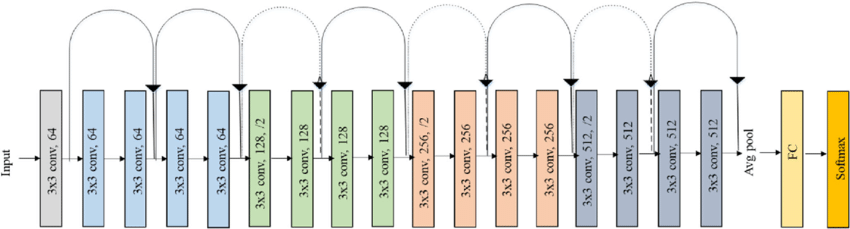
\includegraphics[width=0.9\textwidth]{images/ResNet-18-architecture.png}
    \captionof{figure}{ResNet-18 architecture. Figure taken from \cite{paper-with-resnet-18-figure}.
        The FC is short for Fully Connected layers, and the conv is short for convolutional layers. }
    \label{fig:resnet-18-architecture}
\end{center}


The architecture is implemented PyTorch\cite{PyTorch} and other similar libraries, making it easy to use.


\pagebreak

\printbibliography[title={Litterature}]
\pagebreak
% Start the appendix
\appendix
\part{Appendix}
\chapter{ResNet18 architecture trained with MixUp}\label{appendix:resnet-18-mixup}
This is very heavily inspired by the competetion Kaggle competetion submission by Leon Blume \cite{kaggle-97-model}.

The training was done on DTU high performance computing cluster\cite{dtu-hpc}.
Here a GPU was used, specifically the Tesla V100 16 GB.
\section{Model}
\inputminted{python}{models/resnet_mixup/ham10000_resnet.py}
\section{Output}
\inputminted{python}{models/resnet_mixup/pretty-Output}
\chapter{Ruler saliency maps}\label{appendix:ruler_saliency_maps}
\input{build/saliency_maps/saliency_maps_appendix.tex}
\end{document}